\documentclass[twocolumn]{article}
\usepackage{authblk}
\usepackage[cm]{fullpage}
\usepackage{comment}
\usepackage[square,numbers]{natbib}
\usepackage{graphicx}
\usepackage[subrefformat=parens,labelformat=parens]{subfig}
\usepackage{acronym}
\usepackage{hyperref}
\title{Decision Theoretic Agent Based Modelling: Pregnancy and Alcohol Misuse}
\author{Jonathan Gray\footnote{Corresponding author}}
\author{Jakub Bijak}
\author{Seth Bullock}
\affil{University of Southampton}
\date{\vspace{-5ex}}
\begin{document}
\maketitle
\acrodef{ABM}{Agent Based Model/}
\acrodef{CPT}{Cumulative Prospect Theory}

%Let's say about 750 words. That's 250 on what, 250 on why, 200 on what we found. 50 on what next?

\section{Introduction} %(half page)

Agent Based Modelling, and computational approaches more generally, have been advocated for within the social sciences by many authors (\citep{Axelrod1997, epstein1994growing, agent_zero, gilbert1999simulation, Macy2002a, Resnick,Silverman2011,Silverman2013} are a handful of examples). Despite this, there is a pervasive unease about the use of ABM \citep{Waldherr2013}, which we suggest arises in part from weak theoretical underpinnings. The moving parts of ABMs are often remarkably ad hoc, and poorly specified, based on intuitions about individual behaviour even where the model itself is designed as an expression of a well defined theoretical model. To some extent this may seem inescapable, given that there is no overarching and universal theory of human behaviour. We argue that employing a decision theoretic approach can significantly strengthen the psychological plausibility of ABM, heighten explanatory power, and further that a theoretical grounding to agent behaviour can contribute to development of the underlying theories.

In this work we outline the process of moving from a real world scenario, to a stylised game theoretic representation. The resulting game is then translated to paired decision problems which form the basis of an ABM able to reproduce stylised facts seen in reality.


\section{The Disclosure Game}\label{case} %(half page)

In our model we consider a stylised representation of pregnant women deciding over several appointments what to reveal about their drinking behaviour to their midwives, who must decide whether to refer them to a specialist or continue routine treatment. 
This scenario is readily representable as a form of repeated signalling game \citep{Kreps1987}, where women are privately informed of their drinking type, and may use signals to communicate this (or not) to their midwives. Because alcohol consumption in pregnancy is generally negatively regarded, and can impact on health outcomes for the child, a private type is also assigned to midwives. This determines the extent to which they socially punish a woman for their signalled drinking pattern. Both parties have a common interest in the best health outcome, but potentially clashing interests in that women wish to avoid being stigmatised, and midwives to minimise uneeded referrals.

Rather than approach this explicitly as a game, we instead approach it by transforming into a set of decision problems by treating the game `as if'\footnote{i.e. from the perspective of the agent, since nature is generally disinterested which is not the case here.} against nature \citep{RiosInsua2009}. This permits the use of simple decision rules, and shifts the focus from information acquisition and mental modelling, to decision and action. 

This decision theoretic framing is attractive for several reasons, key amongst which is the potential to offer psychological plausibility. Recent work in neuroeconomics (see particularly \citep{Padoa-Schioppa2006}, and \citep{Rustichini2009} for a more general review) suggests that the concept of a universal currency for comparing the desirability of outcomes in the brain has a solid evidence base.  
From a pragmatic perspective, the decision rules are not computationally demanding, and are modular, demonstrated in this case study by the use of multiple theories with no change to the surrounding model.  In a similar vein, altering the decision problem does not require a reconstruction of the agents. This raises the possibility of effectively training a population of agents in one setting, and subsequently allowing them to use the resultant beliefs in different circumstances. Also appealing is the possibility to contribute to the field of decision theory by providing a convenient test for decision rules, since the validity of the large scale behaviour of the model can be seen as indicative of the capability of the decision rule at the local level.

Four decision rules were considered: (1) simple Bayesian risk minimisation, which attempts to infer the distribution of player types, and likelihood of referral; (2) Cumulative Prospect Theory \citep{Tversky1992} with Bayesian updating, as a well known descriptive theory; (3) a simple lexicographic rule, which uses one reason decision making along the lines of a Fast and Frugal Heuristic \citep{Gigerenzer1996} and considers only the total payoff from a round; and finally (4) a second Bayesian risk minimisation rule which uses equivalent information to the heuristic method in (3).

All four decision rules are able to produce stylised facts identified by \citep{Alvik2006} showing greater concealment by heavy drinkers, and \citep{Phillips2007} reporting a tendency towards more disclosure over appointments (figure \ref{fig_1}). 

The model also incorporates a simple form of information sharing, were following a complete sequence of appointments a player may report their experiences to a randomly selected subset of the population. This leads to significantly divergent behaviour (figure \ref{fig_2}), arising both from the differing rules, and the constrainted problem representation of 3 \& 4. This dichotomy highlights that the nature of the operationalisation of decision making is, in itself, a key decison.

\begin{figure}[h!]{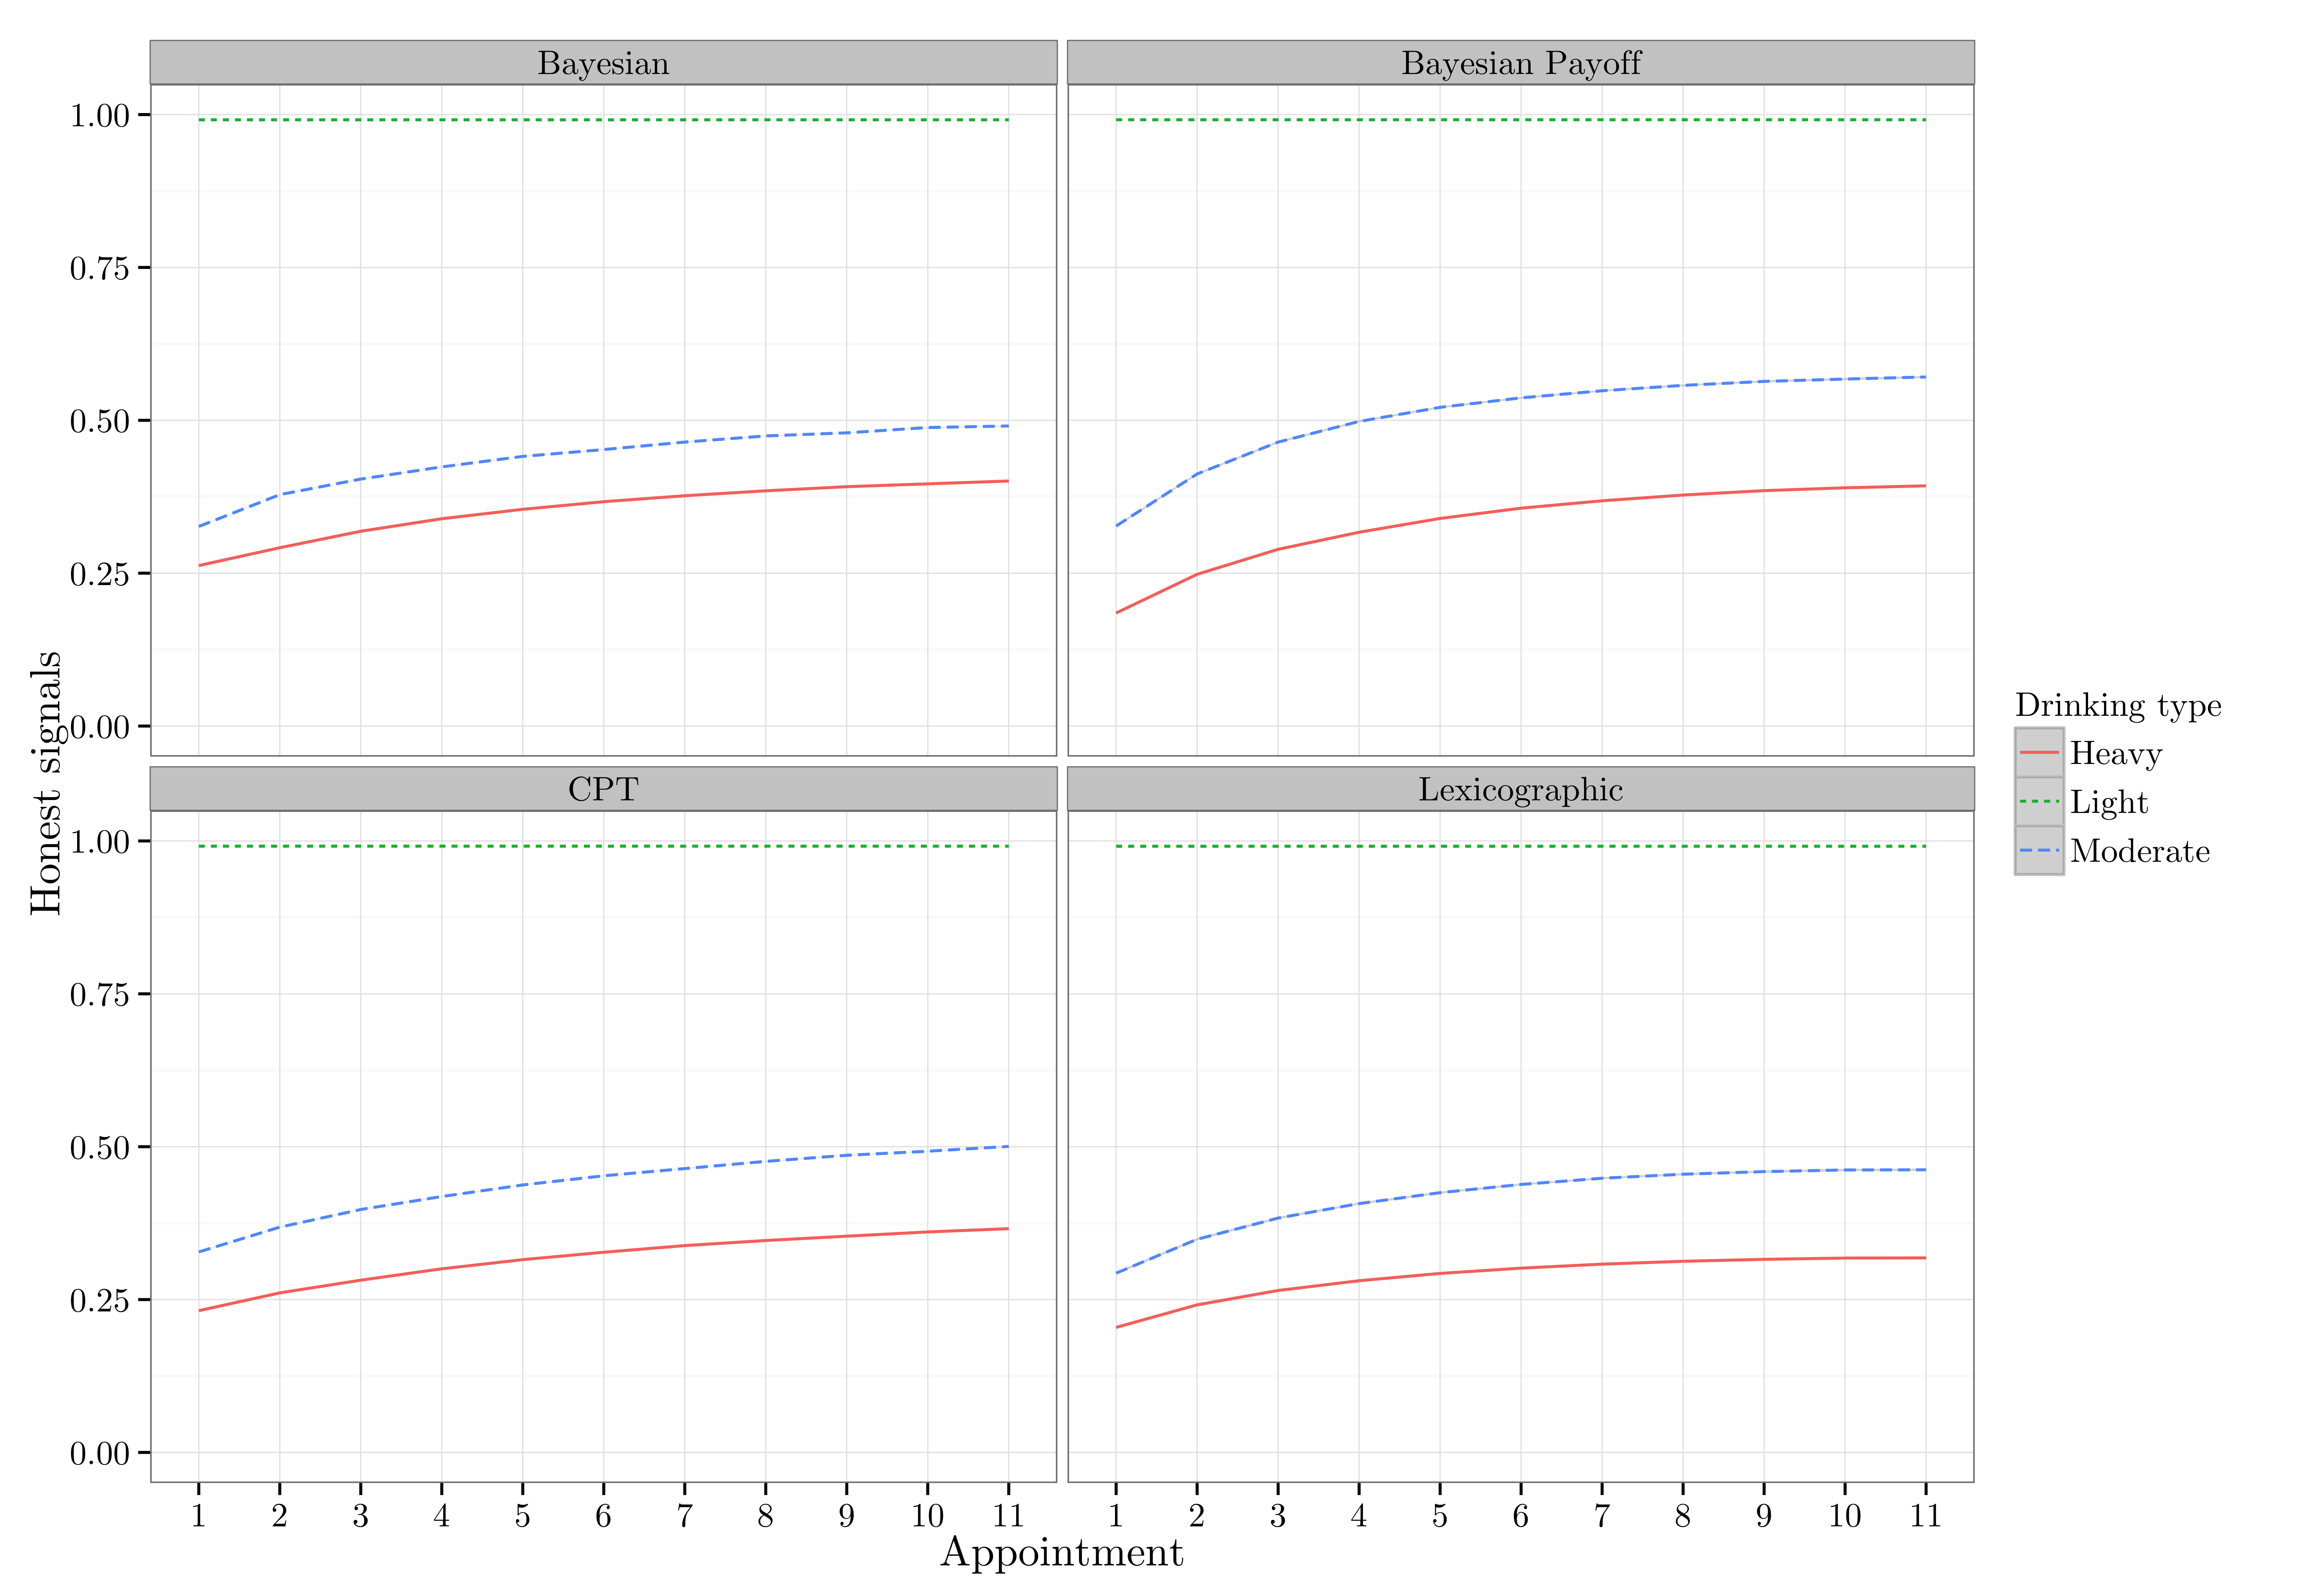
\includegraphics[width=\columnwidth]{honesty_plot}}
	\caption{Decision rules demonstrating increasing honesty signalling over appointments, and greater concealment by heavy drinkers.\label{fig_1}}
\end{figure}

\begin{figure}[h!]{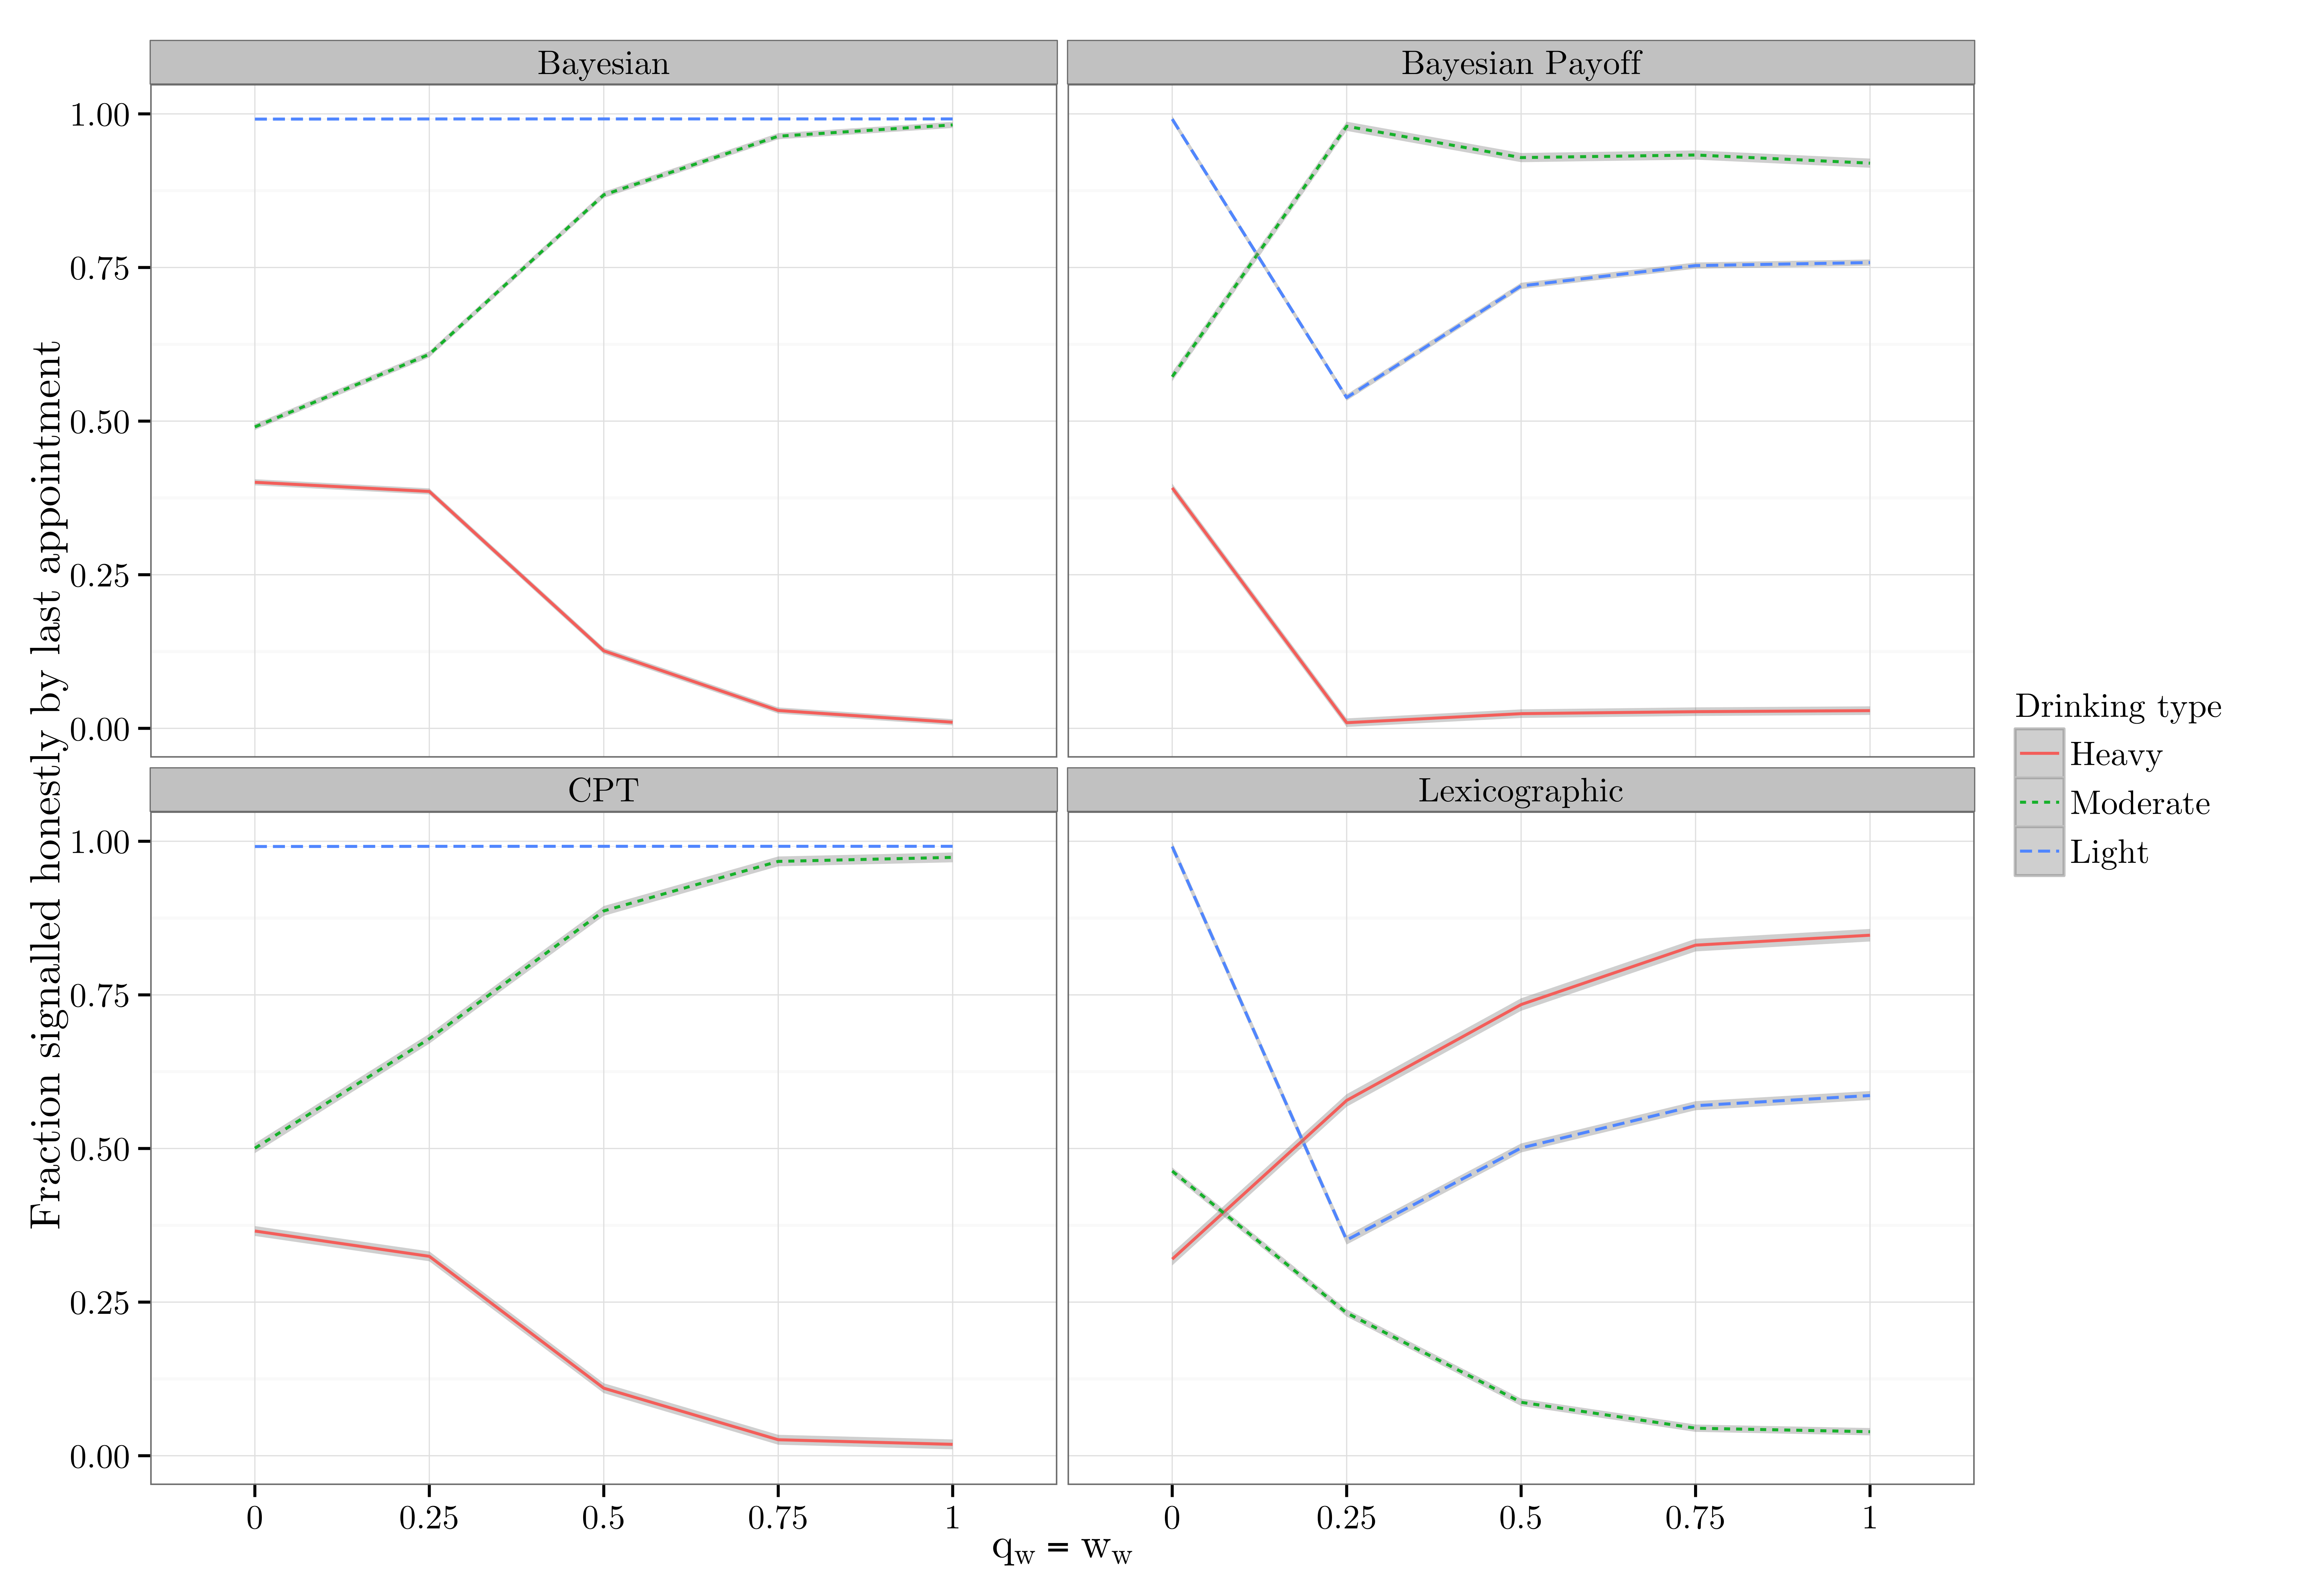
\includegraphics[width=\columnwidth]{honesty_sharing}}
	\caption{Divergence of behaviour under varying degrees of information sharing by women.\label{fig_2}}
\end{figure}
\bibliographystyle{myplainnat}
\bibliography{library}
\end{document}